\documentclass[tikz,border=2pt]{standalone}
\usepackage{amsmath,amssymb}
\usepackage{tikz}
\usetikzlibrary{matrix}

\begin{document}
% The bordered Hessian: the Hessian of the Lagrangian in the x-variables, framed ("bordered")
% by the constraint Jacobian and a zero block for the multipliers.
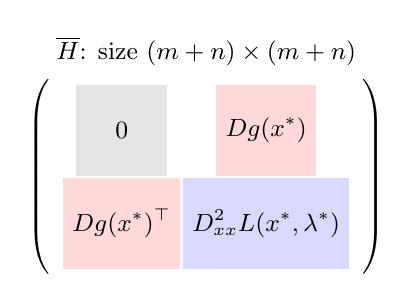
\begin{tikzpicture}[every node/.style={font=\small}]
	\matrix (H) [matrix of math nodes, nodes={minimum size=1.15cm, anchor=center}, left delimiter=(, right delimiter=), column sep=1pt, row sep=1pt] at (0,0) {
		|[fill=gray!20]| 0 & |[fill=red!15]| Dg(x^\ast) \\
		|[fill=red!15]| Dg(x^\ast)^{\top} & |[fill=blue!15]| D^2_{xx}L(x^\ast,\lambda^\ast) \\
	};
	\node[anchor=south] at (H.north) {$\overline{H}$: size $(m+n)\times(m+n)$};
\end{tikzpicture}
\end{document}
